%iffalse
\let\negmedspace\undefined
\let\negthickspace\undefined
\documentclass[journal,12pt,onecolumn]{IEEEtran}
\usepackage{cite}
\usepackage{amsmath,amssymb,amsfonts,amsthm}
\usepackage{algorithmic}
\usepackage{graphicx}
\usepackage{textcomp}
\usepackage{xcolor}
\usepackage{txfonts}
\usepackage{listings}
\usepackage{enumitem}
\usepackage{mathtools}
\usepackage{gensymb}
\usepackage{comment}
\usepackage[breaklinks=true]{hyperref}
\usepackage{tkz-euclide} 
\usepackage{listings}
\usepackage{gvv}      
%\def\inputGnumericTable{}                                 
\usepackage[latin1]{inputenc}                                
\usepackage{color}                                            
\usepackage{array}                                            
\usepackage{longtable}                                       
\usepackage{calc}                                             
\usepackage{multirow}    
\usepackage{hhline}                                           
\usepackage{ifthen}
\usepackage{tikz}

\usepackage{lscape}
\usepackage{tabularx}
\usepackage{array}
\usepackage{float}
\usepackage{multicol}

\newtheorem{theorem}{Theorem}[section]
\newtheorem{problem}{Problem}
\newtheorem{proposition}{Proposition}[section]
\newtheorem{lemma}{Lemma}[section]
\newtheorem{corollary}[theorem]{Corollary}
\newtheorem{example}{Example}[section]
\newtheorem{definition}[problem]{Definition}
\newcommand{\BEQA}{\begin{eqnarray}}
\newcommand{\EEQA}{\end{eqnarray}}
\newcommand{\define}{\stackrel{\triangle}{=}}
\theoremstyle{remark}
\newtheorem{rem}{Remark}

% Marks the beginning of the document
\begin{document}
\bibliographystyle{IEEEtran}
\vspace{3cm}

\title{AE : GATE 2008}
\author{ai24btech11014 \\ Charitha Sri}

\maketitle
\bigskip       
\renewcommand{\thefigure}{\theenumi}
\renewcommand{\thetable}{\theenumi}

\section{ 69-85}

\begin{enumerate}
\item A beam occupies a region $0\leq x \leq L$; $-c \leq y \leq c$; $ -0.5 \leq z \leq 0.5 $ as shown below. The beam can be considered to be in plane stress condition in $x-y$ plane. Airy's stress function for the beam is given as:
      \begin{align}
      \phi \brak{x, y} = -\frac{Px{y}^3}{4{c}^3}+\frac{3Pxy}{4c}
      \end{align}
      where P is a constant.


\begin{center}
\begin{tikzpicture}

    % Coordinates for the points
    \coordinate (O) at (0,0); % Origin
    \coordinate (A) at (8,0); % End of the bar

    % Drawing the bar
    \draw[thick] (O) -- (A);
    \draw[dashed] (O) ++(0,0.3) -- ++(8,0);
    \draw[dashed] (O) ++(0,-0.3) -- ++(8,0);
      \draw[dashed] (O) ++(0, 0.01) -- ++(0, 0.3);
    
    % Force at the end
    \draw[->, thick] (A) -- ++(1,0) node[right] {$x$};
    
    % Marking thickness 'c'
    \draw[<->] (A) ++(0,0.3) -- ++(0,-0.6) node[midway, right] {$c$};

    % Horizontal dimension 'L'
    \draw[<->] (O) ++(0,-0.7) -- ++(8,0) node[midway, below] {$L$};
    
    % y axis
    \draw[->, thick] (O) -- ++(0,-2) node[below] {$y$};
    
    % Labeling point O
    \node at (O) [left] {O};

\end{tikzpicture}
\end{center}

      The above stress function pertains to a 
      \begin{enumerate}
      \item simply supported beam carrying a point load P at mid span 
      \item simply supported beam carrying a uniform distributed load of intensity P per unit length 
      \item cantilever beam clamped at end $x = L$ and carrying a shear load $P$ at $x = 0$
      \item cantilever beam clamped at end $x = 0$ and carrying a shear load $P$ at $x = L$
      \end{enumerate}
\item The equation of motion of a uniform slender beam of length L in flexural vibration is given as $EI
\frac{{\partial}^4 w}{\partial {x}^{4}} + \rho A \frac{{\partial}^{2}}{\partial w {t}^{2}}=0$, where $EI$ is the flexural rigidity, $w$ is the lateral displacement and $\rho A$ is the mass per unit length. The beam is simply supported at the two ends $x =0$ and $x=L$. Assuming the mode shape in fundamental mode to be $\sin\brak{\frac{{\pi x}}{L}}$, the natural frequency in fundamental mode is 
\begin{enumerate}
\begin{multicols}{4}
\item $ 0.5 \sqrt{\frac{EI}{\rho A {L}^{4}}} {\pi}^{2}$
\item $ \sqrt{\frac{EI}{\rho A {L}^{4}}} {\pi}^{2}$
\item $2\sqrt{\frac{EI}{\rho A {L}^{4}}} {\pi}^{2}$
\item $4\sqrt{\frac{EI}{\rho A {L}^{4}}} {\pi}^{2}$
\end{multicols}
\end{enumerate}

\section{Common Data Questions}
\textbf{Common Data Questions 3, 4 and 5}: A two-dimensional state of stress in an isotropic material is given by 
\begin{align}
   \sbrak{\sigma} = c \begin{pmatrix}-8 & 5 \\ 5 & 16\end{pmatrix} MPa
\end{align} 
where c is linearly proportional to the applied loading. The failure stress is $\sigma_{f}=350MPa$ (which is $0.2\%$ offset yield stress)
\item The principal stresses are 
\begin{enumerate}
\begin{multicols}{2}
\item $\sigma_{1} = 17c MPa, \sigma_{2} = -9c MPa$
\item $\sigma_{1} = 9c MPa, \sigma_{2} = 17c MPa$
\item $\sigma_{1} = -17c MPa, \sigma_{2} = -9c MPa$
\item $\sigma_{1} = -17c MPa, \sigma_{2} = 9c MPa$
\end{multicols}
\end{enumerate}

\item  The maximum shear stress is 
\begin{enumerate}
\begin{multicols}{4}
    \item $\tau_{\text{max}}=7c MPa$
    \item $\tau_{\text{max}}=10c MPa$
    \item $\tau_{\text{max}}=13c MPa$
    \item $\tau_{\text{max}}=15c MPa$
\end{multicols}
\end{enumerate}

\item The maximum value of c for safe loading of the structure, based on von-Mises failure criterion is 
\begin{enumerate}
\begin{multicols}{4}
    \item $ 10.2 $
    \item $15.3$
    \item $25.4$
    \item $31.8$
    \end{multicols}
\end{enumerate}

\textbf{Common Data Questions 6 and 7}:A liquid rocket engine with oxidiser to fuel ratio $5:1$ produces a thrust of $1 MN$. The initial mass of the rocket engine is $ 100,000 kg$ and its mass at burn out is $ 10,000kg $. The charracteristic velocity $\vec{C}$ and thrust coefficient $C_{f}$ for the engine are $2386 m/s$  and $1.4$, respectively.

\item The mass flow rate of fuel is 
\begin{enumerate}
\begin{multicols}{4}
    \item $ 300.3 kg/s$
    \item $269.5 kg/s$
    \item $87.4 kg/s$
    \item $49.9 kg/s$
\end{multicols}
\end{enumerate}

\item Neglecting gravity and drag effects, if the initial velocity of the liquid rocket engine is $2.5 km/s $, the velocity of the rocket at burnout is
\begin{enumerate}
\begin{multicols}{4}
    \item $ 1.2 km/s$
    \item $ 2.5 km/s$
    \item $ 10.2 km/s$
    \item $ 11.8 km/s$
 \end{multicols}
\end{enumerate}

\textbf{Linked Answer Questions: 8 and 9}
The following two questions relate to Simpson's rule for approximating the \begin{align}
\int_{a}^{b} f\brak{x} dx \text{on the interval} \sbrak{a, b}
\end{align}

\item Which of the following gives the correct formula for Simpson's rule?
\begin{enumerate}
\begin{multicols}{2}
     \item $ \frac{\brak{ b - a}}{2} \sbrak{ f\brak{b} + f\brak{\frac{a+b}{2}}}$
  \item $ \frac{\brak{ b - a}}{2} \sbrak{ \frac{f\brak{a} +f\brak{b}}{2} + f\brak{\frac{a+b}{2}}}$
  \item $ \frac{\brak{ b - a}}{2} \sbrak{  \frac{f\brak{a} +f\brak{b}}{3} +\frac{4}{3} f\brak{\frac{a+b}{2}}}$
  \item $ \frac{\brak{ b - a}}{2} \sbrak{  \frac{f\brak{a} +f\brak{b}}{3}+ \frac{4}{3}f\brak{\frac{a+b}{2}}}$
 \end{multicols}
\end{enumerate}
\item The percentage error (with respect to the exact solution) in estimation of the integral $\int_{0}^{1} x^{3} dx$ using Simpson's rule 
\begin{enumerate}
\begin{multicols}{4}
    \item $5.3 $
    \item $ 3.5 $
    \item $ 2.8 $
    \item $ 0 $
    \end{multicols}
\end{enumerate}

\textbf{Statement for Linked Answer Questions 10 and 11}: An aircraft has a zero-lift drag coefficient $C_{\text{Do}} = 0.0223$, wing aspect ratio $AR_{w} = 10.0 $, and Oswald's efficiency factor $e = 0.7$
\item The trust required for steady level flight will be minimum when the aircraft operates at a lift coefficient of 
\begin{enumerate}
\begin{multicols}{4}
    \item $ 0.65 $
    \item $ 0.70$
    \item $ 0.75$
    \item $ 0.80$
    \end{multicols}
\end{enumerate}
 \item The glide angle that results in maximum range in a power-off glide is
\begin{enumerate}
\begin{multicols}{4}
    \item $ 1.82 degrees$
    \item $ 2.68 degrees$
    \item $ 3.64 degrees$
    \item $ 5.01 degrees$
    \end{multicols}
\end{enumerate}

\textbf{Statement for Linked Answer Questions 11 and 12}: Consider an unwisted wing of elliptical planform in inviscid incompressible irrotational flow at an angle of attack of 4 degrees. The wing aspect ratio is 7 and the zero lift angle of attack is -2 degrees.

\item The wing lift coefficient $C_{\text{L}}$ is 
\begin{enumerate}
\begin{multicols}{4}
    \item $ 0.66 $
    \item $ 0.51$
    \item $ 0.44$
    \item $ 0.34$
    \end{multicols}
\end{enumerate}
\item The induced drag coefficient of the wing $C_{\text{D}}$ is
\begin{enumerate}
\begin{multicols}{4}
    \item $ 0.0053 $
    \item $ 0.0087 $
    \item $ 0.0118 $
    \item $ 0.0197$
    \end{multicols}
\end{enumerate}

\textbf{Statement for Linked Answer Questions 13 and 14}: A multi-stage axial flow compressor operating at an adiabatic efficiency of $0.9$ develops a total pressure ratio of 11. The total temperature at inlet to the compressor is $335K$ and the stagnation enthalpy rise across each stage is $37 kJ/kg$. Ratio of specific heats is $1.4$ and specific heat at constant pressure is $1.005 kJ/kg K$.
\item The total temperature rise across the compressor is
\begin{enumerate}
\begin{multicols}{4}
    \item $ 310.1K $
    \item $ 366.3K $
    \item $ 392.1K $
    \item $ 405.4K $
    \end{multicols}
\end{enumerate}

\item The total number of stages required are
\begin{enumerate}
\begin{multicols}{4}
    \item $ 9 $
    \item $ 10 $
    \item $ 11 $
    \item $ 12 $
    \end{multicols}
\end{enumerate}

\textbf{Statement for Linked Answer Questions 15 and 16}: An idealized thin walled two cell symmetric box beam is as shown. The shear flows in the walls are due to the applied shear forces $V_{y} = 480 N$, $V_{z} = 300 N$, and a torque M, all acting at the shear center.

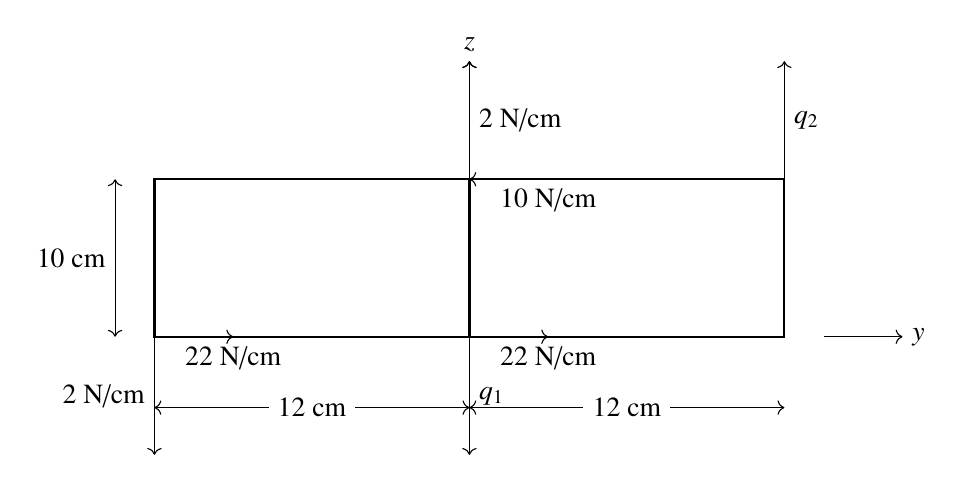
\begin{tikzpicture}


    % Define coordinates for the points
    \coordinate (A) at (0,0);
    \coordinate (B) at (4,0);
    \coordinate (C) at (4,2);
    \coordinate (D) at (0,2);
    \coordinate (E) at (8,0);
    \coordinate (F) at (8,2);

    % Draw the rectangles (two boxes)
    \draw[thick] (A) -- (B) -- (C) -- (D) -- cycle; % Left rectangle
    \draw[thick] (B) -- (E) -- (F) -- (C);          % Right rectangle

    % External force arrows
    \draw[->] (A) -- ++(0,-1.5) node[midway, left] {2 N/cm};  % Bottom left vertical force (2 N/cm)
    \draw[->] (C) -- ++(0,1.5) node[midway, right] {2 N/cm};  % Top left vertical force (2 N/cm)
    \draw[->] (F) -- ++(0,1.5) node[midway, right] {$q_2$};   % Top right unknown force (q2)
    
    % Horizontal force arrows at the bottom
    \draw[->] (A) -- ++(1,0) node[below] {22 N/cm};   % Bottom left horizontal force (22 N/cm)
    \draw[->] (B) -- ++(1,0) node[below] {22 N/cm};   % Bottom right horizontal force (22 N/cm)
    
    % Internal horizontal force between rectangles
    \draw[<-] (C) -- ++(1,0) node[below] {10 N/cm};   % Internal horizontal force (10 N/cm)

    % Vertical force at the right-bottom (q1)
    \draw[->] (B) -- ++(0,-1.5) node[midway, right] {$q_1$};  % Bottom right unknown force (q1)

    % Dimensions
    \draw[<->] (A) ++(0,-0.9) -- ++(4,0) node[midway, fill=white] {12 cm};   % Bottom left length (12 cm)
    \draw[<->] (B) ++(0,-0.9) -- ++(4,0) node[midway, fill=white] {12 cm};   % Bottom right length (12 cm)
    \draw[<->] (D) ++(-0.5,0) -- ++(0,-2) node[midway, left, fill=white] {10 cm};   % Left height (10 cm)

    % Axes
    \draw[->] (8.5,0) -- ++(1,0) node[right] {$y$};   % y-axis
    \draw[->] (4,2.5) -- ++(0,1) node[above] {$z$};   % z-axis



\end{tikzpicture}

\item The shear flows $q_{1}$ and $q_{2}$ are
\begin{enumerate}
\begin{multicols}{2}
    \item $ q_{1} = -2 N/cm\text{,}q_{2} = +22 N/cm$
      \item $ q_{1} = +2 N/cm\text{,}q_{2} = +22 N/cm$
 \item $ q_{1} = +2 N/cm\text{,} q_{2} = -22 N/cm$
\item $ q_{1} = -2 N/cm \text{,}q_{2} = -22 N/cm$

    \end{multicols}
\end{enumerate}
\item The torque M is
\begin{enumerate}
\begin{multicols}{4}
    \item $ 3360 N.cm $
    \item $ 5760 N.cm $
    \item $ 6960 N.cm $
    \item $ 8160 N.cm $
    \end{multicols}
\end{enumerate}


\end{enumerate}
\end{document}
